\section{Aufbau}
\label{sec:Aufbau}
Der Versuchaufbau ist in \autoref{fig:Aufbau} dargestellt und besteht hauptsächlich aus einer Gammaquelle, einem Würfel und einem NaJ-Detektor.
\begin{figure}[H]
    \centering
    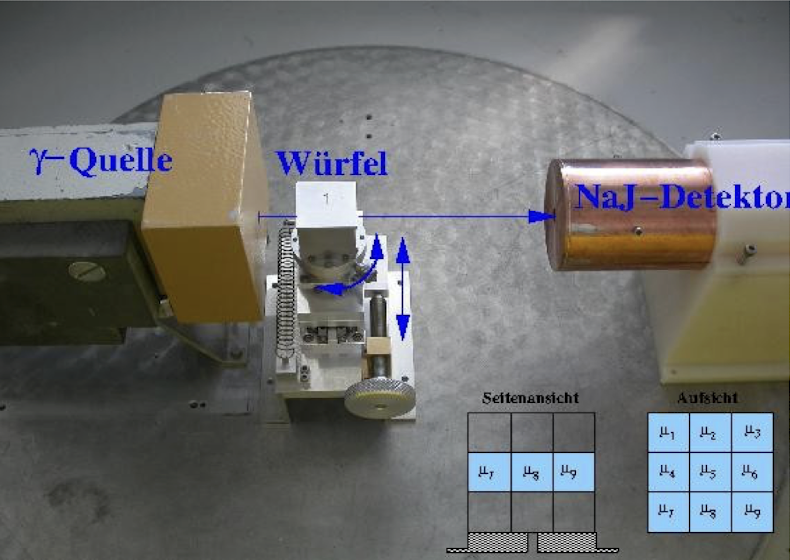
\includegraphics[scale=0.7]{Abbildungen/Aufbau.png}
    \caption{Bild von dem Versuchsaufbau.\cite{V14}}
    \label{fig:Aufbau}
\end{figure}
Die Gammaquelle sendet einen kollimierten Strahl aus, welcher auf den Würfel trifft. 
Der Würfel ist $\qty{3}{\centi\meter} \times \qty{3}{\centi\meter} \times \qty{3}{\centi\meter}$ groß und besteht aus $3 \times 3 \times 3$ Elementarwürfeln, die eime Seitenlänge
von $\qty{1}{\centi\meter}$ besitzen. Die Elementarwürfel werden von einer Aluminiumhülle mit einer Wandstärke von $\qty{1}{\milli\meter}$ umgeben.\\
Es gibt vier unterschiedliche Ausführungen von diesem Würfel. Der erste Würfel besteht nur aus der Aluminiumhülle.
Beim zweiten und dritten Würfel bestehen alle in der Aluminiumhülle enthaltenen Elementarwürfel jeweils nur aus einem Material. Der vierte Würfel besteht aus
einer Mischung von Elementarwürfeln der Materialen des zweiten und dritten Würfels.
Der durchstrahlte Würfel kann um seine z-Achse gedreht werden und senkrecht zur Strahlrichtung verschoben werden.
Der Strahl wird nach dem Durchlaufen des Würfels von einem NaJ-Detektor aufgenommen, wobei die vom Szintillatordetektor erzeugten Pulse von einem Vorverstärker verstärkt werden.
Anschließend werden diese Pulse von einem Multichannelanalyser analysiert, indem das Siganl entsprechend seiner Größe einem Kanal innerhalb des Datensatzes zugeordnet wird.
An einem Spektroskopie Amplifier werde die Detektorspannung und die Vorverstärkerspannung eingestellt und die Diskriminatorschwelle und die Datenaufnahme werden über den Computer und ein 
Programm ausgewertet.


\section{Durchführung}
\label{sec:Durchführung}
Zuerst wird das Spektrum der Quelle bestimmt, ohne Abschwächung des Strahls, also ohne einen Würfel im Strahlengang.
Dabei sollen alle Prozesse des Spektrums identifiziert werden.
Es wird über einem Zeitraum  von $t = \qty{300}{\second}$ gemessen.

Anschließend wird die Messung mit jeweils einem der vier Würfel durchgeführt und die Werte aufgenommen.
Es wird nur die mittlere Schicht des Würfels untersucht, aufgrund von Zeitgründen.
Bei den homogenen Würfeln wird aus vier Richtungen gemessen, der Würfel mit den verschiedenen 
Elementarwürfeln wird aus allen 12 Richtungen gemessen(siehe \autoref{fig:Ausrichtung}).